\documentclass[1p]{elsarticle_modified}
%\bibliographystyle{elsarticle-num}

%\usepackage[colorlinks]{hyperref}
%\usepackage{abbrmath_seonhwa} %\Abb, \Ascr, \Acal ,\Abf, \Afrak
\usepackage{amsfonts}
\usepackage{amssymb}
\usepackage{amsmath}
\usepackage{amsthm}
\usepackage{scalefnt}
\usepackage{amsbsy}
\usepackage{kotex}
\usepackage{caption}
\usepackage{subfig}
\usepackage{color}
\usepackage{graphicx}
\usepackage{xcolor} %% white, black, red, green, blue, cyan, magenta, yellow
\usepackage{float}
\usepackage{setspace}
\usepackage{hyperref}

\usepackage{tikz}
\usetikzlibrary{arrows}

\usepackage{multirow}
\usepackage{array} % fixed length table
\usepackage{hhline}

%%%%%%%%%%%%%%%%%%%%%
\makeatletter
\renewcommand*\env@matrix[1][\arraystretch]{%
	\edef\arraystretch{#1}%
	\hskip -\arraycolsep
	\let\@ifnextchar\new@ifnextchar
	\array{*\c@MaxMatrixCols c}}
\makeatother %https://tex.stackexchange.com/questions/14071/how-can-i-increase-the-line-spacing-in-a-matrix
%%%%%%%%%%%%%%%

\usepackage[normalem]{ulem}

\newcommand{\msout}[1]{\ifmmode\text{\sout{\ensuremath{#1}}}\else\sout{#1}\fi}
%SOURCE: \msout is \stkout macro in https://tex.stackexchange.com/questions/20609/strikeout-in-math-mode

\newcommand{\cancel}[1]{
	\ifmmode
	{\color{red}\msout{#1}}
	\else
	{\color{red}\sout{#1}}
	\fi
}

\newcommand{\add}[1]{
	{\color{blue}\uwave{#1}}
}

\newcommand{\replace}[2]{
	\ifmmode
	{\color{red}\msout{#1}}{\color{blue}\uwave{#2}}
	\else
	{\color{red}\sout{#1}}{\color{blue}\uwave{#2}}
	\fi
}

\newcommand{\Sol}{\mathcal{S}} %segment
\newcommand{\D}{D} %diagram
\newcommand{\A}{\mathcal{A}} %arc


%%%%%%%%%%%%%%%%%%%%%%%%%%%%%5 test

\def\sl{\operatorname{\textup{SL}}(2,\Cbb)}
\def\psl{\operatorname{\textup{PSL}}(2,\Cbb)}
\def\quan{\mkern 1mu \triangleright \mkern 1mu}

\theoremstyle{definition}
\newtheorem{thm}{Theorem}[section]
\newtheorem{prop}[thm]{Proposition}
\newtheorem{lem}[thm]{Lemma}
\newtheorem{ques}[thm]{Question}
\newtheorem{cor}[thm]{Corollary}
\newtheorem{defn}[thm]{Definition}
\newtheorem{exam}[thm]{Example}
\newtheorem{rmk}[thm]{Remark}
\newtheorem{alg}[thm]{Algorithm}

\newcommand{\I}{\sqrt{-1}}
\begin{document}

%\begin{frontmatter}
%
%\title{Boundary parabolic representations of knots up to 8 crossings}
%
%%% Group authors per affiliation:
%\author{Yunhi Cho} 
%\address{Department of Mathematics, University of Seoul, Seoul, Korea}
%\ead{yhcho@uos.ac.kr}
%
%
%\author{Seonhwa Kim} %\fnref{s_kim}}
%\address{Center for Geometry and Physics, Institute for Basic Science, Pohang, 37673, Korea}
%\ead{ryeona17@ibs.re.kr}
%
%\author{Hyuk Kim}
%\address{Department of Mathematical Sciences, Seoul National University, Seoul 08826, Korea}
%\ead{hyukkim@snu.ac.kr}
%
%\author{Seokbeom Yoon}
%\address{Department of Mathematical Sciences, Seoul National University, Seoul, 08826,  Korea}
%\ead{sbyoon15@snu.ac.kr}
%
%\begin{abstract}
%We find all boundary parabolic representation of knots up to 8 crossings.
%
%\end{abstract}
%\begin{keyword}
%    \MSC[2010] 57M25 
%\end{keyword}
%
%\end{frontmatter}

%\linenumbers
%\tableofcontents
%
\newcommand\colored[1]{\textcolor{white}{\rule[-0.35ex]{0.8em}{1.4ex}}\kern-0.8em\color{red} #1}%
%\newcommand\colored[1]{\textcolor{white}{ #1}\kern-2.17ex	\textcolor{white}{ #1}\kern-1.81ex	\textcolor{white}{ #1}\kern-2.15ex\color{red}#1	}

{\Large $\underline{12n_{0817}~(K12n_{0817})}$}

\setlength{\tabcolsep}{10pt}
\renewcommand{\arraystretch}{1.6}
\vspace{1cm}\begin{tabular}{m{100pt}>{\centering\arraybackslash}m{274pt}}
\multirow{5}{120pt}{
	\centering
	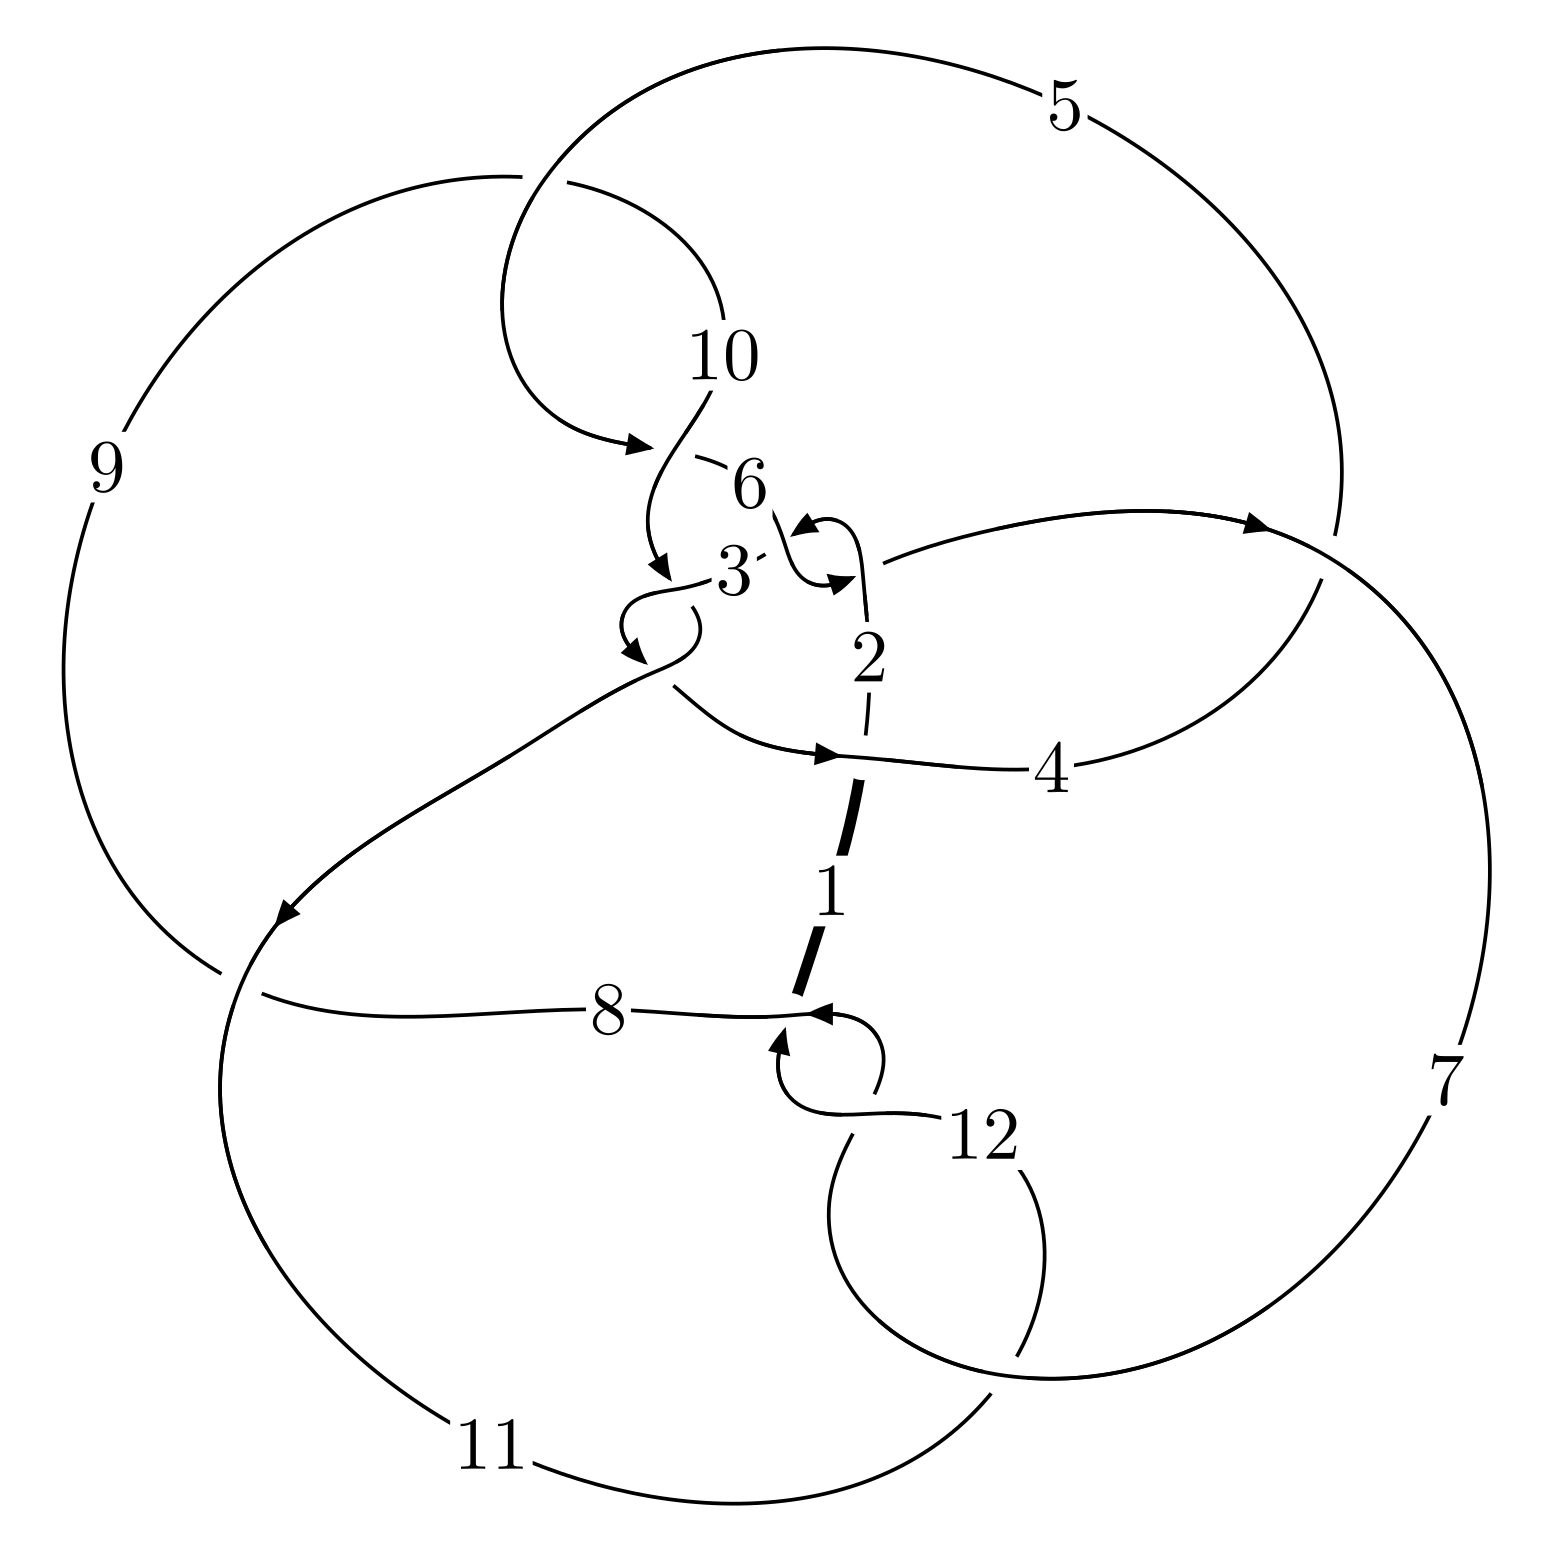
\includegraphics[width=112pt]{../../../GIT/diagram.site/Diagrams/png/2906_12n_0817.png}\\
\ \ \ A knot diagram\footnotemark}&
\allowdisplaybreaks
\textbf{Linearized knot diagam} \\
\cline{2-2}
 &
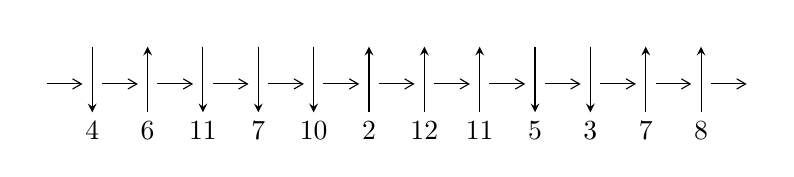
\begin{tikzpicture}[x=20pt, y=17pt]
	% nodes
	\node (C0) at (0, 0) {};
	\node (C1) at (1, 0) {};
	\node (C1U) at (1, +1) {};
	\node (C1D) at (1, -1) {4};

	\node (C2) at (2, 0) {};
	\node (C2U) at (2, +1) {};
	\node (C2D) at (2, -1) {6};

	\node (C3) at (3, 0) {};
	\node (C3U) at (3, +1) {};
	\node (C3D) at (3, -1) {11};

	\node (C4) at (4, 0) {};
	\node (C4U) at (4, +1) {};
	\node (C4D) at (4, -1) {7};

	\node (C5) at (5, 0) {};
	\node (C5U) at (5, +1) {};
	\node (C5D) at (5, -1) {10};

	\node (C6) at (6, 0) {};
	\node (C6U) at (6, +1) {};
	\node (C6D) at (6, -1) {2};

	\node (C7) at (7, 0) {};
	\node (C7U) at (7, +1) {};
	\node (C7D) at (7, -1) {12};

	\node (C8) at (8, 0) {};
	\node (C8U) at (8, +1) {};
	\node (C8D) at (8, -1) {11};

	\node (C9) at (9, 0) {};
	\node (C9U) at (9, +1) {};
	\node (C9D) at (9, -1) {5};

	\node (C10) at (10, 0) {};
	\node (C10U) at (10, +1) {};
	\node (C10D) at (10, -1) {3};

	\node (C11) at (11, 0) {};
	\node (C11U) at (11, +1) {};
	\node (C11D) at (11, -1) {7};

	\node (C12) at (12, 0) {};
	\node (C12U) at (12, +1) {};
	\node (C12D) at (12, -1) {8};
	\node (C13) at (13, 0) {};

	% arrows
	\draw[->,>={angle 60}]
	(C0) edge (C1) (C1) edge (C2) (C2) edge (C3) (C3) edge (C4) (C4) edge (C5) (C5) edge (C6) (C6) edge (C7) (C7) edge (C8) (C8) edge (C9) (C9) edge (C10) (C10) edge (C11) (C11) edge (C12) (C12) edge (C13) ;	\draw[->,>=stealth]
	(C1U) edge (C1D) (C2D) edge (C2U) (C3U) edge (C3D) (C4U) edge (C4D) (C5U) edge (C5D) (C6D) edge (C6U) (C7D) edge (C7U) (C8D) edge (C8U) (C9U) edge (C9D) (C10U) edge (C10D) (C11D) edge (C11U) (C12D) edge (C12U) ;
	\end{tikzpicture} \\
\hhline{~~} \\& 
\textbf{Solving Sequence} \\ \cline{2-2} 
 &
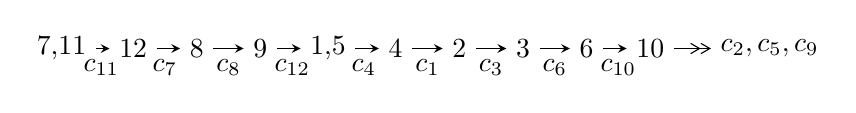
\begin{tikzpicture}[x=23pt, y=7pt]
	% node
	\node (A0) at (-1/8, 0) {7,11};
	\node (A1) at (1, 0) {12};
	\node (A2) at (2, 0) {8};
	\node (A3) at (3, 0) {9};
	\node (A4) at (65/16, 0) {1,5};
	\node (A5) at (41/8, 0) {4};
	\node (A6) at (49/8, 0) {2};
	\node (A7) at (57/8, 0) {3};
	\node (A8) at (65/8, 0) {6};
	\node (A9) at (73/8, 0) {10};
	\node (C1) at (1/2, -1) {$c_{11}$};
	\node (C2) at (3/2, -1) {$c_{7}$};
	\node (C3) at (5/2, -1) {$c_{8}$};
	\node (C4) at (7/2, -1) {$c_{12}$};
	\node (C5) at (37/8, -1) {$c_{4}$};
	\node (C6) at (45/8, -1) {$c_{1}$};
	\node (C7) at (53/8, -1) {$c_{3}$};
	\node (C8) at (61/8, -1) {$c_{6}$};
	\node (C9) at (69/8, -1) {$c_{10}$};
	\node (A10) at (11, 0) {$c_{2},c_{5},c_{9}$};

	% edge
	\draw[->,>=stealth]	
	(A0) edge (A1) (A1) edge (A2) (A2) edge (A3) (A3) edge (A4) (A4) edge (A5) (A5) edge (A6) (A6) edge (A7) (A7) edge (A8) (A8) edge (A9) ;
	\draw[->>,>={angle 60}]	
	(A9) edge (A10);
\end{tikzpicture} \\ 

\end{tabular} \\

\footnotetext{
The image of knot diagram is generated by the software ``\textbf{Draw programme}" developed by Andrew Bartholomew(\url{http://www.layer8.co.uk/maths/draw/index.htm\#Running-draw}), where we modified some parts for our purpose(\url{https://github.com/CATsTAILs/LinksPainter}).
}\phantom \\ \newline 
\centering \textbf{Ideals for irreducible components\footnotemark of $X_{\text{par}}$} 
 
\begin{align*}
I^u_{1}&=\langle 
-139 u^{18}+1059 u^{17}+\cdots+4 b-764,\;-87 u^{18}+677 u^{17}+\cdots+8 a-508,\;u^{19}-9 u^{18}+\cdots+12 u-8\rangle \\
I^u_{2}&=\langle 
2 u^{12}+2 u^{11}-15 u^{10}-12 u^9+43 u^8+27 u^7-53 u^6-26 u^5+20 u^4+10 u^3+6 u^2+b-4 u-2,\\
\phantom{I^u_{2}}&\phantom{= \langle  }u^{10}+u^9-7 u^8-6 u^7+18 u^6+13 u^5-18 u^4-10 u^3+2 u^2+a+4,\\
\phantom{I^u_{2}}&\phantom{= \langle  }u^{13}+2 u^{12}-7 u^{11}-14 u^{10}+19 u^9+38 u^8-22 u^7-46 u^6+6 u^5+20 u^4+7 u^3+u^2-5 u-1\rangle \\
I^u_{3}&=\langle 
5 a^5 u^2-7 a^4 u^2+\cdots-11 a+26,\;2 a^5 u^2+a^4 u^2+\cdots+95 a+46,\;u^3+u^2-2 u-1\rangle \\
\\
\end{align*}
\raggedright * 3 irreducible components of $\dim_{\mathbb{C}}=0$, with total 50 representations.\\
\footnotetext{All coefficients of polynomials are rational numbers. But the coefficients are sometimes approximated in decimal forms when there is not enough margin.}
\newpage
\renewcommand{\arraystretch}{1}
\centering \section*{I. $I^u_{1}= \langle -139 u^{18}+1059 u^{17}+\cdots+4 b-764,\;-87 u^{18}+677 u^{17}+\cdots+8 a-508,\;u^{19}-9 u^{18}+\cdots+12 u-8 \rangle$}
\flushleft \textbf{(i) Arc colorings}\\
\begin{tabular}{m{7pt} m{180pt} m{7pt} m{180pt} }
\flushright $a_{7}=$&$\begin{pmatrix}0\\u\end{pmatrix}$ \\
\flushright $a_{11}=$&$\begin{pmatrix}1\\0\end{pmatrix}$ \\
\flushright $a_{12}=$&$\begin{pmatrix}1\\- u^2\end{pmatrix}$ \\
\flushright $a_{8}=$&$\begin{pmatrix}u\\- u^3+u\end{pmatrix}$ \\
\flushright $a_{9}=$&$\begin{pmatrix}- u^3+2 u\\- u^3+u\end{pmatrix}$ \\
\flushright $a_{1}=$&$\begin{pmatrix}- u^2+1\\u^4-2 u^2\end{pmatrix}$ \\
\flushright $a_{5}=$&$\begin{pmatrix}10.8750 u^{18}-84.6250 u^{17}+\cdots-51.7500 u+63.5000\\\frac{139}{4} u^{18}-\frac{1059}{4} u^{17}+\cdots-159 u+191\end{pmatrix}$ \\
\flushright $a_{4}=$&$\begin{pmatrix}10.8750 u^{18}-84.6250 u^{17}+\cdots-51.7500 u+63.5000\\\frac{87}{4} u^{18}-\frac{611}{4} u^{17}+\cdots-87 u+85\end{pmatrix}$ \\
\flushright $a_{2}=$&$\begin{pmatrix}-\frac{63}{8} u^{18}+\frac{465}{8} u^{17}+\cdots+\frac{135}{4} u-38\\-\frac{1}{4} u^{18}+\frac{7}{4} u^{17}+\cdots+\frac{1}{2} u-1\end{pmatrix}$ \\
\flushright $a_{3}=$&$\begin{pmatrix}32.6250 u^{18}-237.375 u^{17}+\cdots-138.750 u+148.500\\\frac{87}{4} u^{18}-\frac{611}{4} u^{17}+\cdots-87 u+85\end{pmatrix}$ \\
\flushright $a_{6}=$&$\begin{pmatrix}\frac{169}{8} u^{18}-\frac{1229}{8} u^{17}+\cdots-\frac{181}{2} u+96\\6 u^{18}-\frac{85}{2} u^{17}+\cdots-\frac{47}{2} u+25\end{pmatrix}$ \\
\flushright $a_{10}=$&$\begin{pmatrix}\frac{1}{8} u^{18}-\frac{7}{8} u^{17}+\cdots+\frac{3}{4} u+1\\\frac{1}{4} u^{18}-\frac{7}{4} u^{17}+\cdots-\frac{1}{2} u+1\end{pmatrix}$\\&\end{tabular}
\flushleft \textbf{(ii) Obstruction class $= -1$}\\~\\
\flushleft \textbf{(iii) Cusp Shapes $= -25 u^{18}+174 u^{17}-365 u^{16}-25 u^{15}+771 u^{14}+163 u^{13}-1928 u^{12}+630 u^{11}+1143 u^{10}+293 u^9-304 u^8-532 u^7-1600 u^6+1277 u^5+1032 u^4-324 u^3-389 u^2+90 u-94$}\\~\\
\newpage\renewcommand{\arraystretch}{1}
\flushleft \textbf{(iv) u-Polynomials at the component}\newline \\
\begin{tabular}{m{50pt}|m{274pt}}
Crossings & \hspace{64pt}u-Polynomials at each crossing \\
\hline $$\begin{aligned}c_{1},c_{4}\end{aligned}$$&$\begin{aligned}
&u^{19}+u^{18}+\cdots+12 u+1
\end{aligned}$\\
\hline $$\begin{aligned}c_{2},c_{6}\end{aligned}$$&$\begin{aligned}
&u^{19}-8 u^{18}+\cdots-52 u+8
\end{aligned}$\\
\hline $$\begin{aligned}c_{3},c_{5},c_{9}\\c_{10}\end{aligned}$$&$\begin{aligned}
&u^{19}- u^{18}+\cdots-2 u-1
\end{aligned}$\\
\hline $$\begin{aligned}c_{7},c_{11},c_{12}\end{aligned}$$&$\begin{aligned}
&u^{19}-9 u^{18}+\cdots+12 u-8
\end{aligned}$\\
\hline $$\begin{aligned}c_{8}\end{aligned}$$&$\begin{aligned}
&u^{19}+27 u^{18}+\cdots+27116 u+3512
\end{aligned}$\\
\hline
\end{tabular}\\~\\
\newpage\renewcommand{\arraystretch}{1}
\flushleft \textbf{(v) Riley Polynomials at the component}\newline \\
\begin{tabular}{m{50pt}|m{274pt}}
Crossings & \hspace{64pt}Riley Polynomials at each crossing \\
\hline $$\begin{aligned}c_{1},c_{4}\end{aligned}$$&$\begin{aligned}
&y^{19}+35 y^{18}+\cdots+42 y-1
\end{aligned}$\\
\hline $$\begin{aligned}c_{2},c_{6}\end{aligned}$$&$\begin{aligned}
&y^{19}+16 y^{18}+\cdots-48 y-64
\end{aligned}$\\
\hline $$\begin{aligned}c_{3},c_{5},c_{9}\\c_{10}\end{aligned}$$&$\begin{aligned}
&y^{19}-11 y^{18}+\cdots+10 y-1
\end{aligned}$\\
\hline $$\begin{aligned}c_{7},c_{11},c_{12}\end{aligned}$$&$\begin{aligned}
&y^{19}-23 y^{18}+\cdots-432 y-64
\end{aligned}$\\
\hline $$\begin{aligned}c_{8}\end{aligned}$$&$\begin{aligned}
&y^{19}-43 y^{18}+\cdots+4640976 y-12334144
\end{aligned}$\\
\hline
\end{tabular}\\~\\
\newpage\flushleft \textbf{(vi) Complex Volumes and Cusp Shapes}
$$\begin{array}{c|c|c}  
\text{Solutions to }I^u_{1}& \I (\text{vol} + \sqrt{-1}CS) & \text{Cusp shape}\\
 \hline 
\begin{aligned}
u &= -0.091188 + 0.966333 I \\
a &= \phantom{-}0.733877 - 0.319784 I \\
b &= \phantom{-}0.211486 - 0.489342 I\end{aligned}
 & -6.48169 + 2.66282 I & -2.52143 - 2.56509 I \\ \hline\begin{aligned}
u &= -0.091188 - 0.966333 I \\
a &= \phantom{-}0.733877 + 0.319784 I \\
b &= \phantom{-}0.211486 + 0.489342 I\end{aligned}
 & -6.48169 - 2.66282 I & -2.52143 + 2.56509 I \\ \hline\begin{aligned}
u &= -0.904144 + 0.517931 I \\
a &= \phantom{-}0.706601 - 1.068440 I \\
b &= \phantom{-}0.218968 - 0.639966 I\end{aligned}
 & \phantom{-}2.53064 - 4.01875 I & \phantom{-}1.69485 + 6.55873 I \\ \hline\begin{aligned}
u &= -0.904144 - 0.517931 I \\
a &= \phantom{-}0.706601 + 1.068440 I \\
b &= \phantom{-}0.218968 + 0.639966 I\end{aligned}
 & \phantom{-}2.53064 + 4.01875 I & \phantom{-}1.69485 - 6.55873 I \\ \hline\begin{aligned}
u &= \phantom{-}1.19835\phantom{ +0.000000I} \\
a &= \phantom{-}0.103232\phantom{ +0.000000I} \\
b &= \phantom{-}0.623676\phantom{ +0.000000I}\end{aligned}
 & \phantom{-}2.53576\phantom{ +0.000000I} & \phantom{-}4.52770\phantom{ +0.000000I} \\ \hline\begin{aligned}
u &= -0.634175 + 0.351711 I \\
a &= -1.29575 + 1.15797 I \\
b &= -0.392189 + 0.643839 I\end{aligned}
 & \phantom{-}0.91268 + 1.32361 I & -5.06829 + 3.42198 I \\ \hline\begin{aligned}
u &= -0.634175 - 0.351711 I \\
a &= -1.29575 - 1.15797 I \\
b &= -0.392189 - 0.643839 I\end{aligned}
 & \phantom{-}0.91268 - 1.32361 I & -5.06829 - 3.42198 I \\ \hline\begin{aligned}
u &= -1.060850 + 0.713165 I \\
a &= -0.549004 + 0.898836 I \\
b &= -0.176307 + 0.591660 I\end{aligned}
 & -3.53037 - 8.31890 I & -1.40883 + 6.39242 I \\ \hline\begin{aligned}
u &= -1.060850 - 0.713165 I \\
a &= -0.549004 - 0.898836 I \\
b &= -0.176307 - 0.591660 I\end{aligned}
 & -3.53037 + 8.31890 I & -1.40883 - 6.39242 I \\ \hline\begin{aligned}
u &= \phantom{-}1.289480 + 0.424662 I \\
a &= \phantom{-}0.114699 - 0.319331 I \\
b &= -0.272999 - 0.853707 I\end{aligned}
 & -2.23583 + 2.25035 I & -0.46692 - 2.77886 I\\
 \hline 
 \end{array}$$\newpage$$\begin{array}{c|c|c}  
\text{Solutions to }I^u_{1}& \I (\text{vol} + \sqrt{-1}CS) & \text{Cusp shape}\\
 \hline 
\begin{aligned}
u &= \phantom{-}1.289480 - 0.424662 I \\
a &= \phantom{-}0.114699 + 0.319331 I \\
b &= -0.272999 + 0.853707 I\end{aligned}
 & -2.23583 - 2.25035 I & -0.46692 + 2.77886 I \\ \hline\begin{aligned}
u &= \phantom{-}0.103961 + 0.369644 I \\
a &= -0.936993 - 0.305312 I \\
b &= -0.163488 + 0.354518 I\end{aligned}
 & -0.056986 + 0.926042 I & -1.11794 - 7.21094 I \\ \hline\begin{aligned}
u &= \phantom{-}0.103961 - 0.369644 I \\
a &= -0.936993 + 0.305312 I \\
b &= -0.163488 - 0.354518 I\end{aligned}
 & -0.056986 - 0.926042 I & -1.11794 + 7.21094 I \\ \hline\begin{aligned}
u &= \phantom{-}1.67359 + 0.17987 I \\
a &= \phantom{-}0.094930 + 1.113270 I \\
b &= \phantom{-}0.63844 + 2.62086 I\end{aligned}
 & \phantom{-}9.08712 + 1.06966 I & -0.590577 - 0.693151 I \\ \hline\begin{aligned}
u &= \phantom{-}1.67359 - 0.17987 I \\
a &= \phantom{-}0.094930 - 1.113270 I \\
b &= \phantom{-}0.63844 - 2.62086 I\end{aligned}
 & \phantom{-}9.08712 - 1.06966 I & -0.590577 + 0.693151 I \\ \hline\begin{aligned}
u &= \phantom{-}1.73838 + 0.18173 I \\
a &= \phantom{-}0.101477 - 1.233980 I \\
b &= -0.15677 - 2.84161 I\end{aligned}
 & \phantom{-}11.82410 + 7.02626 I & \phantom{-}2.32832 - 4.17154 I \\ \hline\begin{aligned}
u &= \phantom{-}1.73838 - 0.18173 I \\
a &= \phantom{-}0.101477 + 1.233980 I \\
b &= -0.15677 + 2.84161 I\end{aligned}
 & \phantom{-}11.82410 - 7.02626 I & \phantom{-}2.32832 + 4.17154 I \\ \hline\begin{aligned}
u &= \phantom{-}1.78576 + 0.20016 I \\
a &= -0.271457 + 1.238060 I \\
b &= -0.21898 + 2.80030 I\end{aligned}
 & \phantom{-}6.42171 + 12.16180 I & -0.61302 - 5.43087 I \\ \hline\begin{aligned}
u &= \phantom{-}1.78576 - 0.20016 I \\
a &= -0.271457 - 1.238060 I \\
b &= -0.21898 - 2.80030 I\end{aligned}
 & \phantom{-}6.42171 - 12.16180 I & -0.61302 + 5.43087 I\\
 \hline 
 \end{array}$$\newpage\newpage\renewcommand{\arraystretch}{1}
\centering \section*{II. $I^u_{2}= \langle 2 u^{12}+2 u^{11}+\cdots+b-2,\;u^{10}+u^9+\cdots+a+4,\;u^{13}+2 u^{12}+\cdots-5 u-1 \rangle$}
\flushleft \textbf{(i) Arc colorings}\\
\begin{tabular}{m{7pt} m{180pt} m{7pt} m{180pt} }
\flushright $a_{7}=$&$\begin{pmatrix}0\\u\end{pmatrix}$ \\
\flushright $a_{11}=$&$\begin{pmatrix}1\\0\end{pmatrix}$ \\
\flushright $a_{12}=$&$\begin{pmatrix}1\\- u^2\end{pmatrix}$ \\
\flushright $a_{8}=$&$\begin{pmatrix}u\\- u^3+u\end{pmatrix}$ \\
\flushright $a_{9}=$&$\begin{pmatrix}- u^3+2 u\\- u^3+u\end{pmatrix}$ \\
\flushright $a_{1}=$&$\begin{pmatrix}- u^2+1\\u^4-2 u^2\end{pmatrix}$ \\
\flushright $a_{5}=$&$\begin{pmatrix}- u^{10}- u^9+7 u^8+6 u^7-18 u^6-13 u^5+18 u^4+10 u^3-2 u^2-4\\-2 u^{12}-2 u^{11}+\cdots+4 u+2\end{pmatrix}$ \\
\flushright $a_{4}=$&$\begin{pmatrix}- u^{10}- u^9+7 u^8+6 u^7-18 u^6-13 u^5+18 u^4+10 u^3-2 u^2-4\\- u^{12}- u^{11}+\cdots+4 u+2\end{pmatrix}$ \\
\flushright $a_{2}=$&$\begin{pmatrix}- u^{10}- u^9+7 u^8+6 u^7-18 u^6-14 u^5+18 u^4+14 u^3-3 u^2-4 u-3\\u^4-3 u^2+1\end{pmatrix}$ \\
\flushright $a_{3}=$&$\begin{pmatrix}- u^{12}- u^{11}+7 u^{10}+5 u^9-18 u^8-8 u^7+17 u^6+3 u^5-4 u^2+4 u-2\\- u^{12}- u^{11}+\cdots+4 u+2\end{pmatrix}$ \\
\flushright $a_{6}=$&$\begin{pmatrix}- u^{11}- u^{10}+7 u^9+5 u^8-18 u^7-8 u^6+17 u^5+2 u^4+4 u^2-5 u\\u^7-5 u^5+7 u^3+u^2-2 u-1\end{pmatrix}$ \\
\flushright $a_{10}=$&$\begin{pmatrix}- u^{12}-2 u^{11}+\cdots+2 u+5\\- u^3+2 u-1\end{pmatrix}$\\&\end{tabular}
\flushleft \textbf{(ii) Obstruction class $= 1$}\\~\\
\flushleft \textbf{(iii) Cusp Shapes $= -3 u^{11}-7 u^{10}+17 u^9+43 u^8-33 u^7-95 u^6+13 u^5+73 u^4+23 u^3+6 u^2-14 u-14$}\\~\\
\newpage\renewcommand{\arraystretch}{1}
\flushleft \textbf{(iv) u-Polynomials at the component}\newline \\
\begin{tabular}{m{50pt}|m{274pt}}
Crossings & \hspace{64pt}u-Polynomials at each crossing \\
\hline $$\begin{aligned}c_{1},c_{4}\end{aligned}$$&$\begin{aligned}
&u^{13}+u^{12}+\cdots+3 u^2-1
\end{aligned}$\\
\hline $$\begin{aligned}c_{2}\end{aligned}$$&$\begin{aligned}
&u^{13}- u^{12}+\cdots+2 u+1
\end{aligned}$\\
\hline $$\begin{aligned}c_{3},c_{9}\end{aligned}$$&$\begin{aligned}
&u^{13}+u^{12}-4 u^{11}-4 u^{10}+6 u^9+5 u^8-2 u^7+4 u^6-2 u^5-14 u^4+7 u^2+1
\end{aligned}$\\
\hline $$\begin{aligned}c_{5},c_{10}\end{aligned}$$&$\begin{aligned}
&u^{13}- u^{12}-4 u^{11}+4 u^{10}+6 u^9-5 u^8-2 u^7-4 u^6-2 u^5+14 u^4-7 u^2-1
\end{aligned}$\\
\hline $$\begin{aligned}c_{6}\end{aligned}$$&$\begin{aligned}
&u^{13}+u^{12}+\cdots+2 u-1
\end{aligned}$\\
\hline $$\begin{aligned}c_{7}\end{aligned}$$&$\begin{aligned}
&u^{13}-2 u^{12}+\cdots-5 u+1
\end{aligned}$\\
\hline $$\begin{aligned}c_{8}\end{aligned}$$&$\begin{aligned}
&u^{13}+6 u^{12}+\cdots+u+1
\end{aligned}$\\
\hline $$\begin{aligned}c_{11},c_{12}\end{aligned}$$&$\begin{aligned}
&u^{13}+2 u^{12}+\cdots-5 u-1
\end{aligned}$\\
\hline
\end{tabular}\\~\\
\newpage\renewcommand{\arraystretch}{1}
\flushleft \textbf{(v) Riley Polynomials at the component}\newline \\
\begin{tabular}{m{50pt}|m{274pt}}
Crossings & \hspace{64pt}Riley Polynomials at each crossing \\
\hline $$\begin{aligned}c_{1},c_{4}\end{aligned}$$&$\begin{aligned}
&y^{13}+5 y^{12}+\cdots+6 y-1
\end{aligned}$\\
\hline $$\begin{aligned}c_{2},c_{6}\end{aligned}$$&$\begin{aligned}
&y^{13}+13 y^{12}+\cdots+18 y-1
\end{aligned}$\\
\hline $$\begin{aligned}c_{3},c_{5},c_{9}\\c_{10}\end{aligned}$$&$\begin{aligned}
&y^{13}-9 y^{12}+\cdots-14 y-1
\end{aligned}$\\
\hline $$\begin{aligned}c_{7},c_{11},c_{12}\end{aligned}$$&$\begin{aligned}
&y^{13}-18 y^{12}+\cdots+27 y-1
\end{aligned}$\\
\hline $$\begin{aligned}c_{8}\end{aligned}$$&$\begin{aligned}
&y^{13}-26 y^{12}+\cdots+43 y-1
\end{aligned}$\\
\hline
\end{tabular}\\~\\
\newpage\flushleft \textbf{(vi) Complex Volumes and Cusp Shapes}
$$\begin{array}{c|c|c}  
\text{Solutions to }I^u_{2}& \I (\text{vol} + \sqrt{-1}CS) & \text{Cusp shape}\\
 \hline 
\begin{aligned}
u &= \phantom{-}0.820152 + 0.104400 I \\
a &= \phantom{-}0.753200 + 1.119880 I \\
b &= \phantom{-}0.305571 + 0.530288 I\end{aligned}
 & \phantom{-}1.34031 - 1.84544 I & \phantom{-}2.80039 + 5.64574 I \\ \hline\begin{aligned}
u &= \phantom{-}0.820152 - 0.104400 I \\
a &= \phantom{-}0.753200 - 1.119880 I \\
b &= \phantom{-}0.305571 - 0.530288 I\end{aligned}
 & \phantom{-}1.34031 + 1.84544 I & \phantom{-}2.80039 - 5.64574 I \\ \hline\begin{aligned}
u &= -1.26705\phantom{ +0.000000I} \\
a &= -0.390134\phantom{ +0.000000I} \\
b &= -1.85106\phantom{ +0.000000I}\end{aligned}
 & -0.232440\phantom{ +0.000000I} & \phantom{-}0.645970\phantom{ +0.000000I} \\ \hline\begin{aligned}
u &= -1.300200 + 0.250560 I \\
a &= \phantom{-}0.343272 - 0.374017 I \\
b &= \phantom{-}1.63014 - 0.54583 I\end{aligned}
 & -4.74439 - 5.27325 I & -1.78132 + 3.84852 I \\ \hline\begin{aligned}
u &= -1.300200 - 0.250560 I \\
a &= \phantom{-}0.343272 + 0.374017 I \\
b &= \phantom{-}1.63014 + 0.54583 I\end{aligned}
 & -4.74439 + 5.27325 I & -1.78132 - 3.84852 I \\ \hline\begin{aligned}
u &= \phantom{-}1.35503\phantom{ +0.000000I} \\
a &= \phantom{-}0.699592\phantom{ +0.000000I} \\
b &= \phantom{-}0.402528\phantom{ +0.000000I}\end{aligned}
 & \phantom{-}1.54960\phantom{ +0.000000I} & -4.46630\phantom{ +0.000000I} \\ \hline\begin{aligned}
u &= -0.162080 + 0.555123 I \\
a &= -0.32922 + 1.58092 I \\
b &= -0.924848 + 0.088801 I\end{aligned}
 & -8.52981 + 2.40351 I & -9.03747 - 0.70595 I \\ \hline\begin{aligned}
u &= -0.162080 - 0.555123 I \\
a &= -0.32922 - 1.58092 I \\
b &= -0.924848 - 0.088801 I\end{aligned}
 & -8.52981 - 2.40351 I & -9.03747 + 0.70595 I \\ \hline\begin{aligned}
u &= \phantom{-}1.48038 + 0.34329 I \\
a &= -0.744111 + 0.018385 I \\
b &= -0.450757 - 0.029628 I\end{aligned}
 & -2.98672 + 1.03297 I & -3.12657 + 1.51158 I \\ \hline\begin{aligned}
u &= \phantom{-}1.48038 - 0.34329 I \\
a &= -0.744111 - 0.018385 I \\
b &= -0.450757 + 0.029628 I\end{aligned}
 & -2.98672 - 1.03297 I & -3.12657 - 1.51158 I\\
 \hline 
 \end{array}$$\newpage$$\begin{array}{c|c|c}  
\text{Solutions to }I^u_{2}& \I (\text{vol} + \sqrt{-1}CS) & \text{Cusp shape}\\
 \hline 
\begin{aligned}
u &= -1.78337 + 0.04448 I \\
a &= -0.115269 + 1.138540 I \\
b &= -0.34421 + 2.57894 I\end{aligned}
 & \phantom{-}11.19350 + 0.95284 I & \phantom{-}1.091372 - 0.413941 I \\ \hline\begin{aligned}
u &= -1.78337 - 0.04448 I \\
a &= -0.115269 - 1.138540 I \\
b &= -0.34421 - 2.57894 I\end{aligned}
 & \phantom{-}11.19350 - 0.95284 I & \phantom{-}1.091372 + 0.413941 I \\ \hline\begin{aligned}
u &= -0.197734\phantom{ +0.000000I} \\
a &= -4.12519\phantom{ +0.000000I} \\
b &= \phantom{-}1.01673\phantom{ +0.000000I}\end{aligned}
 & -3.73260\phantom{ +0.000000I} & -11.0720\phantom{ +0.000000I}\\
 \hline 
 \end{array}$$\newpage\newpage\renewcommand{\arraystretch}{1}
\centering \section*{III. $I^u_{3}= \langle 5 a^5 u^2-7 a^4 u^2+\cdots-11 a+26,\;2 a^5 u^2+a^4 u^2+\cdots+95 a+46,\;u^3+u^2-2 u-1 \rangle$}
\flushleft \textbf{(i) Arc colorings}\\
\begin{tabular}{m{7pt} m{180pt} m{7pt} m{180pt} }
\flushright $a_{7}=$&$\begin{pmatrix}0\\u\end{pmatrix}$ \\
\flushright $a_{11}=$&$\begin{pmatrix}1\\0\end{pmatrix}$ \\
\flushright $a_{12}=$&$\begin{pmatrix}1\\- u^2\end{pmatrix}$ \\
\flushright $a_{8}=$&$\begin{pmatrix}u\\u^2- u-1\end{pmatrix}$ \\
\flushright $a_{9}=$&$\begin{pmatrix}u^2-1\\u^2- u-1\end{pmatrix}$ \\
\flushright $a_{1}=$&$\begin{pmatrix}- u^2+1\\u^2- u-1\end{pmatrix}$ \\
\flushright $a_{5}=$&$\begin{pmatrix}a\\-0.178571 a^{5} u^{2}+0.250000 a^{4} u^{2}+\cdots+0.392857 a-0.928571\end{pmatrix}$ \\
\flushright $a_{4}=$&$\begin{pmatrix}a\\-0.178571 a^{5} u^{2}+0.250000 a^{4} u^{2}+\cdots+0.392857 a-0.928571\end{pmatrix}$ \\
\flushright $a_{2}=$&$\begin{pmatrix}-0.214286 a^{5} u^{2}-0.250000 a^{4} u^{2}+\cdots+0.0714286 a+1.28571\\\frac{15}{28} a^5 u^2+\frac{1}{2} a^4 u^2+\cdots+\frac{1}{14} a+\frac{2}{7}\end{pmatrix}$ \\
\flushright $a_{3}=$&$\begin{pmatrix}-0.178571 a^{5} u^{2}+0.250000 a^{4} u^{2}+\cdots+1.39286 a-0.928571\\-0.178571 a^{5} u^{2}+0.250000 a^{4} u^{2}+\cdots+0.392857 a-0.928571\end{pmatrix}$ \\
\flushright $a_{6}=$&$\begin{pmatrix}-0.0357143 a^{5} u^{2}-0.500000 a^{4} u^{2}+\cdots-1.32143 a+0.214286\\\frac{1}{14} a^5 u^2-\frac{1}{4} a^4 u^2+\cdots-\frac{5}{14} a+\frac{4}{7}\end{pmatrix}$ \\
\flushright $a_{10}=$&$\begin{pmatrix}\frac{3}{14} a^5 u^2+\frac{1}{4} a^4 u^2+\cdots-\frac{1}{14} a-\frac{9}{7}\\0.535714 a^{5} u^{2}+0.500000 a^{4} u^{2}+\cdots+0.0714286 a-1.71429\end{pmatrix}$\\&\end{tabular}
\flushleft \textbf{(ii) Obstruction class $= -1$}\\~\\
\flushleft \textbf{(iii) Cusp Shapes $= -\frac{10}{7} a^5 u^2-\frac{16}{7} a^5 u+a^4 u^2-\frac{5}{7} a^5+3 a^4 u-\frac{3}{7} a^3 u^2+a^4+\frac{33}{7} a^3 u-\frac{11}{7} a^2 u^2+\frac{16}{7} a^3-\frac{5}{7} a^2 u-\frac{5}{7} u^2 a+\frac{5}{7} a^2+\frac{13}{7} a u-\frac{6}{7} u^2-\frac{13}{7} a+\frac{10}{7} u+\frac{32}{7}$}\\~\\
\newpage\renewcommand{\arraystretch}{1}
\flushleft \textbf{(iv) u-Polynomials at the component}\newline \\
\begin{tabular}{m{50pt}|m{274pt}}
Crossings & \hspace{64pt}u-Polynomials at each crossing \\
\hline $$\begin{aligned}c_{1},c_{4}\end{aligned}$$&$\begin{aligned}
&u^{18}- u^{17}+\cdots-16 u-8
\end{aligned}$\\
\hline $$\begin{aligned}c_{2},c_{6}\end{aligned}$$&$\begin{aligned}
&(u^3+u^2+2 u+1)^6
\end{aligned}$\\
\hline $$\begin{aligned}c_{3},c_{5},c_{9}\\c_{10}\end{aligned}$$&$\begin{aligned}
&u^{18}- u^{17}+\cdots+64 u-8
\end{aligned}$\\
\hline $$\begin{aligned}c_{7},c_{11},c_{12}\end{aligned}$$&$\begin{aligned}
&(u^3+u^2-2 u-1)^6
\end{aligned}$\\
\hline $$\begin{aligned}c_{8}\end{aligned}$$&$\begin{aligned}
&(u^3-3 u^2-4 u-1)^6
\end{aligned}$\\
\hline
\end{tabular}\\~\\
\newpage\renewcommand{\arraystretch}{1}
\flushleft \textbf{(v) Riley Polynomials at the component}\newline \\
\begin{tabular}{m{50pt}|m{274pt}}
Crossings & \hspace{64pt}Riley Polynomials at each crossing \\
\hline $$\begin{aligned}c_{1},c_{4}\end{aligned}$$&$\begin{aligned}
&y^{18}+19 y^{17}+\cdots-3424 y+64
\end{aligned}$\\
\hline $$\begin{aligned}c_{2},c_{6}\end{aligned}$$&$\begin{aligned}
&(y^3+3 y^2+2 y-1)^6
\end{aligned}$\\
\hline $$\begin{aligned}c_{3},c_{5},c_{9}\\c_{10}\end{aligned}$$&$\begin{aligned}
&y^{18}-5 y^{17}+\cdots-2784 y+64
\end{aligned}$\\
\hline $$\begin{aligned}c_{7},c_{11},c_{12}\end{aligned}$$&$\begin{aligned}
&(y^3-5 y^2+6 y-1)^6
\end{aligned}$\\
\hline $$\begin{aligned}c_{8}\end{aligned}$$&$\begin{aligned}
&(y^3-17 y^2+10 y-1)^6
\end{aligned}$\\
\hline
\end{tabular}\\~\\
\newpage\flushleft \textbf{(vi) Complex Volumes and Cusp Shapes}
$$\begin{array}{c|c|c}  
\text{Solutions to }I^u_{3}& \I (\text{vol} + \sqrt{-1}CS) & \text{Cusp shape}\\
 \hline 
\begin{aligned}
u &= \phantom{-}1.24698\phantom{ +0.000000I} \\
a &= -0.922052 + 0.388981 I \\
b &= -1.215350 - 0.381464 I\end{aligned}
 & -1.61418 + 2.82812 I & -1.50976 - 2.97945 I \\ \hline\begin{aligned}
u &= \phantom{-}1.24698\phantom{ +0.000000I} \\
a &= -0.922052 - 0.388981 I \\
b &= -1.215350 + 0.381464 I\end{aligned}
 & -1.61418 - 2.82812 I & -1.50976 + 2.97945 I \\ \hline\begin{aligned}
u &= \phantom{-}1.24698\phantom{ +0.000000I} \\
a &= \phantom{-}0.608898 + 0.654820 I \\
b &= -0.365738 + 0.960730 I\end{aligned}
 & -1.61418 - 2.82812 I & -1.50976 + 2.97945 I \\ \hline\begin{aligned}
u &= \phantom{-}1.24698\phantom{ +0.000000I} \\
a &= \phantom{-}0.608898 - 0.654820 I \\
b &= -0.365738 - 0.960730 I\end{aligned}
 & -1.61418 + 2.82812 I & -1.50976 - 2.97945 I \\ \hline\begin{aligned}
u &= \phantom{-}1.24698\phantom{ +0.000000I} \\
a &= \phantom{-}0.445706\phantom{ +0.000000I} \\
b &= \phantom{-}0.852713\phantom{ +0.000000I}\end{aligned}
 & \phantom{-}2.52340\phantom{ +0.000000I} & \phantom{-}5.01950\phantom{ +0.000000I} \\ \hline\begin{aligned}
u &= \phantom{-}1.24698\phantom{ +0.000000I} \\
a &= -0.176294\phantom{ +0.000000I} \\
b &= \phantom{-}0.507529\phantom{ +0.000000I}\end{aligned}
 & \phantom{-}2.52340\phantom{ +0.000000I} & \phantom{-}5.01950\phantom{ +0.000000I} \\ \hline\begin{aligned}
u &= -0.445042\phantom{ +0.000000I} \\
a &= -0.405582\phantom{ +0.000000I} \\
b &= -1.37094\phantom{ +0.000000I}\end{aligned}
 & -3.11638\phantom{ +0.000000I} & \phantom{-}5.01950\phantom{ +0.000000I} \\ \hline\begin{aligned}
u &= -0.445042\phantom{ +0.000000I} \\
a &= \phantom{-}0.43074 + 1.96960 I \\
b &= \phantom{-}1.62616 + 0.09419 I\end{aligned}
 & -7.25396 + 2.82812 I & -1.50976 - 2.97945 I \\ \hline\begin{aligned}
u &= -0.445042\phantom{ +0.000000I} \\
a &= \phantom{-}0.43074 - 1.96960 I \\
b &= \phantom{-}1.62616 - 0.09419 I\end{aligned}
 & -7.25396 - 2.82812 I & -1.50976 + 2.97945 I \\ \hline\begin{aligned}
u &= -0.445042\phantom{ +0.000000I} \\
a &= -2.65086\phantom{ +0.000000I} \\
b &= \phantom{-}0.429626\phantom{ +0.000000I}\end{aligned}
 & -3.11638\phantom{ +0.000000I} & \phantom{-}5.01950\phantom{ +0.000000I}\\
 \hline 
 \end{array}$$\newpage$$\begin{array}{c|c|c}  
\text{Solutions to }I^u_{3}& \I (\text{vol} + \sqrt{-1}CS) & \text{Cusp shape}\\
 \hline 
\begin{aligned}
u &= -0.445042\phantom{ +0.000000I} \\
a &= \phantom{-}3.12194 + 1.04628 I \\
b &= -0.532013 + 0.834636 I\end{aligned}
 & -7.25396 + 2.82812 I & -1.50976 - 2.97945 I \\ \hline\begin{aligned}
u &= -0.445042\phantom{ +0.000000I} \\
a &= \phantom{-}3.12194 - 1.04628 I \\
b &= -0.532013 - 0.834636 I\end{aligned}
 & -7.25396 - 2.82812 I & -1.50976 + 2.97945 I \\ \hline\begin{aligned}
u &= -1.80194\phantom{ +0.000000I} \\
a &= -0.411551 + 0.882060 I \\
b &= -0.43781 + 2.39534 I\end{aligned}
 & \phantom{-}9.66536 + 2.82812 I & -1.50976 - 2.97945 I \\ \hline\begin{aligned}
u &= -1.80194\phantom{ +0.000000I} \\
a &= -0.411551 - 0.882060 I \\
b &= -0.43781 - 2.39534 I\end{aligned}
 & \phantom{-}9.66536 - 2.82812 I & -1.50976 + 2.97945 I \\ \hline\begin{aligned}
u &= -1.80194\phantom{ +0.000000I} \\
a &= \phantom{-}0.261196 + 1.163730 I \\
b &= \phantom{-}0.16798 + 2.61487 I\end{aligned}
 & \phantom{-}13.8029\phantom{ +0.000000I} & \phantom{-}5.01951 + 0. I\phantom{ +0.000000I} \\ \hline\begin{aligned}
u &= -1.80194\phantom{ +0.000000I} \\
a &= \phantom{-}0.261196 - 1.163730 I \\
b &= \phantom{-}0.16798 - 2.61487 I\end{aligned}
 & \phantom{-}13.8029\phantom{ +0.000000I} & \phantom{-}5.01951 + 0. I\phantom{ +0.000000I} \\ \hline\begin{aligned}
u &= -1.80194\phantom{ +0.000000I} \\
a &= -0.195655 + 1.397520 I \\
b &= \phantom{-}0.04731 + 2.72683 I\end{aligned}
 & \phantom{-}9.66536 - 2.82812 I & -1.50976 + 2.97945 I \\ \hline\begin{aligned}
u &= -1.80194\phantom{ +0.000000I} \\
a &= -0.195655 - 1.397520 I \\
b &= \phantom{-}0.04731 - 2.72683 I\end{aligned}
 & \phantom{-}9.66536 + 2.82812 I & -1.50976 - 2.97945 I\\
 \hline 
 \end{array}$$\newpage
\newpage\renewcommand{\arraystretch}{1}
\centering \section*{ IV. u-Polynomials}
\begin{tabular}{m{50pt}|m{274pt}}
Crossings & \hspace{64pt}u-Polynomials at each crossing \\
\hline $$\begin{aligned}c_{1},c_{4}\end{aligned}$$&$\begin{aligned}
&(u^{13}+u^{12}+\cdots+3 u^2-1)(u^{18}- u^{17}+\cdots-16 u-8)\\
&\cdot(u^{19}+u^{18}+\cdots+12 u+1)
\end{aligned}$\\
\hline $$\begin{aligned}c_{2}\end{aligned}$$&$\begin{aligned}
&((u^3+u^2+2 u+1)^6)(u^{13}- u^{12}+\cdots+2 u+1)\\
&\cdot(u^{19}-8 u^{18}+\cdots-52 u+8)
\end{aligned}$\\
\hline $$\begin{aligned}c_{3},c_{9}\end{aligned}$$&$\begin{aligned}
&(u^{13}+u^{12}-4 u^{11}-4 u^{10}+6 u^9+5 u^8-2 u^7+4 u^6-2 u^5-14 u^4+7 u^2+1)\\
&\cdot(u^{18}- u^{17}+\cdots+64 u-8)(u^{19}- u^{18}+\cdots-2 u-1)
\end{aligned}$\\
\hline $$\begin{aligned}c_{5},c_{10}\end{aligned}$$&$\begin{aligned}
&(u^{13}- u^{12}-4 u^{11}+4 u^{10}+6 u^9-5 u^8-2 u^7-4 u^6-2 u^5+14 u^4-7 u^2-1)\\
&\cdot(u^{18}- u^{17}+\cdots+64 u-8)(u^{19}- u^{18}+\cdots-2 u-1)
\end{aligned}$\\
\hline $$\begin{aligned}c_{6}\end{aligned}$$&$\begin{aligned}
&((u^3+u^2+2 u+1)^6)(u^{13}+u^{12}+\cdots+2 u-1)\\
&\cdot(u^{19}-8 u^{18}+\cdots-52 u+8)
\end{aligned}$\\
\hline $$\begin{aligned}c_{7}\end{aligned}$$&$\begin{aligned}
&((u^3+u^2-2 u-1)^6)(u^{13}-2 u^{12}+\cdots-5 u+1)\\
&\cdot(u^{19}-9 u^{18}+\cdots+12 u-8)
\end{aligned}$\\
\hline $$\begin{aligned}c_{8}\end{aligned}$$&$\begin{aligned}
&((u^3-3 u^2-4 u-1)^6)(u^{13}+6 u^{12}+\cdots+u+1)\\
&\cdot(u^{19}+27 u^{18}+\cdots+27116 u+3512)
\end{aligned}$\\
\hline $$\begin{aligned}c_{11},c_{12}\end{aligned}$$&$\begin{aligned}
&((u^3+u^2-2 u-1)^6)(u^{13}+2 u^{12}+\cdots-5 u-1)\\
&\cdot(u^{19}-9 u^{18}+\cdots+12 u-8)
\end{aligned}$\\
\hline
\end{tabular}\newpage\renewcommand{\arraystretch}{1}
\centering \section*{ V. Riley Polynomials}
\begin{tabular}{m{50pt}|m{274pt}}
Crossings & \hspace{64pt}Riley Polynomials at each crossing \\
\hline $$\begin{aligned}c_{1},c_{4}\end{aligned}$$&$\begin{aligned}
&(y^{13}+5 y^{12}+\cdots+6 y-1)(y^{18}+19 y^{17}+\cdots-3424 y+64)\\
&\cdot(y^{19}+35 y^{18}+\cdots+42 y-1)
\end{aligned}$\\
\hline $$\begin{aligned}c_{2},c_{6}\end{aligned}$$&$\begin{aligned}
&((y^3+3 y^2+2 y-1)^6)(y^{13}+13 y^{12}+\cdots+18 y-1)\\
&\cdot(y^{19}+16 y^{18}+\cdots-48 y-64)
\end{aligned}$\\
\hline $$\begin{aligned}c_{3},c_{5},c_{9}\\c_{10}\end{aligned}$$&$\begin{aligned}
&(y^{13}-9 y^{12}+\cdots-14 y-1)(y^{18}-5 y^{17}+\cdots-2784 y+64)\\
&\cdot(y^{19}-11 y^{18}+\cdots+10 y-1)
\end{aligned}$\\
\hline $$\begin{aligned}c_{7},c_{11},c_{12}\end{aligned}$$&$\begin{aligned}
&((y^3-5 y^2+6 y-1)^6)(y^{13}-18 y^{12}+\cdots+27 y-1)\\
&\cdot(y^{19}-23 y^{18}+\cdots-432 y-64)
\end{aligned}$\\
\hline $$\begin{aligned}c_{8}\end{aligned}$$&$\begin{aligned}
&((y^3-17 y^2+10 y-1)^6)(y^{13}-26 y^{12}+\cdots+43 y-1)\\
&\cdot(y^{19}-43 y^{18}+\cdots+4640976 y-12334144)
\end{aligned}$\\
\hline
\end{tabular}
\vskip 2pc
\end{document}